\documentclass{article}

\usepackage{geometry}
 \geometry{
 a4paper,
 total={170mm,257mm},
 left=20mm,
 top=20mm
 }
\usepackage{float}
\usepackage{graphicx}
\usepackage{indentfirst}
\usepackage{hyperref}

\graphicspath{ {./images/} }
\renewcommand*\contentsname{Daftar Isi}
\renewcommand{\figurename}{Figur}
\renewcommand{\tablename}{Tabel}

\begin{document}
	\begin{titlepage}
		\begin{center}
			
			\null
			{
				\huge \bfseries Tugas Praktikum Pengembangan Perangkat Lunak}\\
			[1cm]
			{\LARGE Business Process KataHati}\\
			
			\vspace{2cm}
			
			\begin{figure}[H]
				\centering
				
\includegraphics[width=200px]{/HitamPutih.jpg}
			\end{figure}
			
			\vspace{3cm}
			
			{\Large 
				Disusun oleh Kelompok YapaYapaHuy} {\Large :\\
				\vspace{0.5cm}
				Ardacandra Subiantoro (18/427572/PA/18532)\\
				Chrystian (18/430257/PA/18770)\\
				Juandito Batara Kuncoro (18/427582/PA/18542)\\
			}
			
			
			\vspace{2cm}
			
			{\normalsize \bfseries
				PROGRAM STUDI S1 ILMU KOMPUTER\\
				DEPARTEMEN ILMU KOMPUTER DAN ELEKTRONIKA\\
				FAKULTAS MATEMATIKA DAN ILMU PENGETAHUAN ALAM\\
				UNIVERSITAS GADJAH MADA\\
				YOGYAKARTA\\
				\vspace{0.2cm}
				2020
			}
			
		\end{center}
	\end{titlepage}

	\newpage
	\pagenumbering{arabic}
	
	\section{Deskripsi Permasalahan}
	\par
	Keadaan pandemi COVID-19 menyebabkan banyak mahasiswa kekurangan interaksi sosial, membuat mereka tidak dapat memenuhi kebutuhan berinteraksi sosial, sehingga dapat menyebabkan stres berlebih dan kurangnya produktivitas. Tujuan program ini membantu mahasiswa yang mengalami masalah mental oleh karena keadaan pandemi untuk menerima saran dan bantuan profesional.
	\par
	Untuk memenuhi kebutuhan tersebut desain perangkat lunak harus memiliki tingkat aksesibilitas yang tinggi untuk dapat meraih dan diketahui oleh mahasiswa yang bermasalah tersebut. Dengan profesional ahli, sistem harus dapat mengatur pertemuan melakukan penjadwalan dan serta menghubungkan profesional dengan mahasiswa bermasalah secara cepat, tepat dan efisien.
	
	\section{Bisnis Proses}
	
	\section{Proses Design}
	\begin{enumerate}
		\item Proses Pendaftaran : mahasiswa mendaftar dan melakukan proses verifikasi.
		\item Proses Pengisian Form : mahasiswa mengisi form untuk  klasifikasi masalah yang mereka alami, lalu mereka diarahkan kepada profesional yang sesuai.
		\item Proses Penjadwalan : mahasiswa memilih jadwal untuk berinteraksi dengan tenaga profesional sesuai waktu yang tersedia.
		\item Proses Interaksi : mahasiswa interaksi dengan profesional dengan media seperti chat.
		\item Proses Sharing Group : mahasiswa dapat bergabung ke dalam chat room berisi mahasiswa-mahasiswa lain yang memiliki masalah serupa.
	\end{enumerate}
	
	\begin{figure}[!h]
		\centering	
		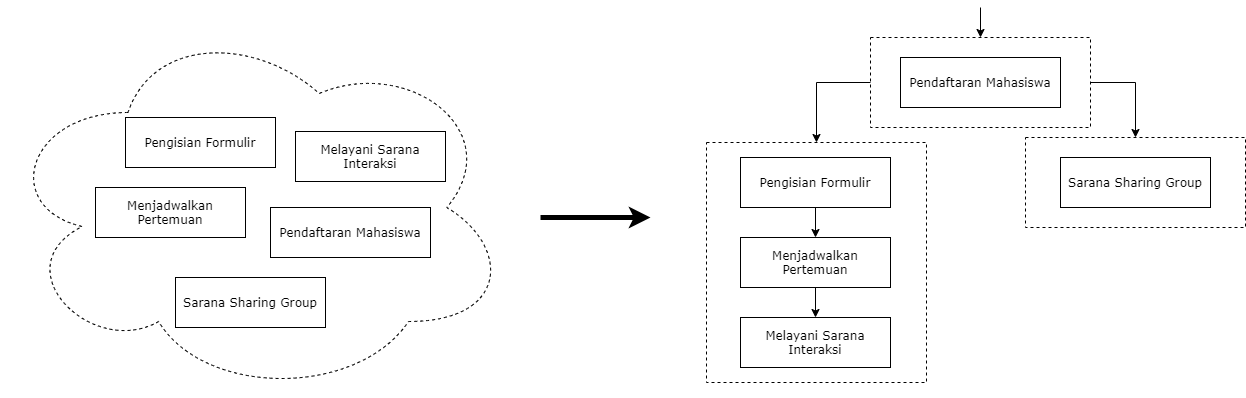
\includegraphics[width=500px]{/diagram/diagram_processes.png}
		\caption{Diagram Pembagian Subscope pada Sistem}
	\end{figure}
	\section{Spesifikasi User}
	\begin{enumerate}
		\item Admin : karyawan yang dapat mengkonfigurasikan sistem, termasuk proses penjadwalan, manajemen database, menjadi moderator chat room.
		\item Mahasiswa : pengguna website yang fasih dengan komputer dan sedang membutuhkan bantuan secara mental.
		\item Profesional : tenaga profesional di bidang kesehatan mental yang dapat memberikan bantuan berupa saran-saran kepada mahasiswa yang mengalami masalah mental.
	\end{enumerate}
	
\end{document}